\documentclass[10pt]{article}
\usepackage[a4paper, margin=0.7in, top=0.6in, bottom=0.6in]{geometry}
\usepackage[T1]{fontenc}
\usepackage{lmodern}
\usepackage{xcolor}
\usepackage{tikz}
\usetikzlibrary{positioning, calc, backgrounds, shapes.geometric}
\usepackage{enumitem}

% Color definitions
\definecolor{timelineblue}{RGB}{41, 98, 255}
\definecolor{optimgreen}{RGB}{0, 150, 80}
\definecolor{conforange}{RGB}{230, 126, 34}
\definecolor{ongoingblue}{RGB}{52, 152, 219}
\definecolor{warnred}{RGB}{192, 57, 43}
\definecolor{lightblue}{RGB}{230, 243, 255}
\definecolor{collabgray}{RGB}{128, 128, 128}

% Category dots
\newcommand{\optmark}{\textcolor{optimgreen}{$\bullet$}}
\newcommand{\confmark}{\textcolor{conforange}{$\bullet$}}
\newcommand{\collabmark}{\textcolor{collabgray}{$\bullet$}}

% Speedup badge
\newcommand{\speedup}[1]{\tikz[baseline=(X.base)]{\node[fill=optimgreen!20, draw=optimgreen, rounded corners=2pt, inner sep=2pt, font=\small\bfseries] (X) {\textcolor{optimgreen}{#1}};}}

% Conference highlight
\newcommand{\conf}[1]{\textcolor{conforange}{\textbf{#1}}}

% Warning text
\newcommand{\warn}[1]{\textcolor{warnred}{#1}}

\setlist[itemize]{leftmargin=1.2em, itemsep=1pt, parsep=1pt, topsep=2pt}

\pagestyle{empty}

\begin{document}

% Title
\begin{center}
{\Large\bfseries GPU Track Reconstruction Optimization Timeline}\\[0.3em]
{\normalsize November 2024 -- January 2026}
\end{center}

\vspace{0.8em}

% Timeline using TikZ
\begin{tikzpicture}[remember picture, overlay]
  % Ongoing work sidebar (2025.9 to 2026.1) - positioned on right margin
  \fill[ongoingblue, opacity=0.12, rounded corners=3pt]
    ([xshift=0.35in, yshift=-4.05in]current page.north east) rectangle
    ([xshift=0.05in, yshift=-10.35in]current page.north east);
  \node[rotate=90, font=\footnotesize\itshape, text=ongoingblue, anchor=south]
    at ([xshift=0.2in, yshift=-7.2in]current page.north east)
    {NCU Profile Flow Optimization (Ongoing)};
\end{tikzpicture}

\noindent
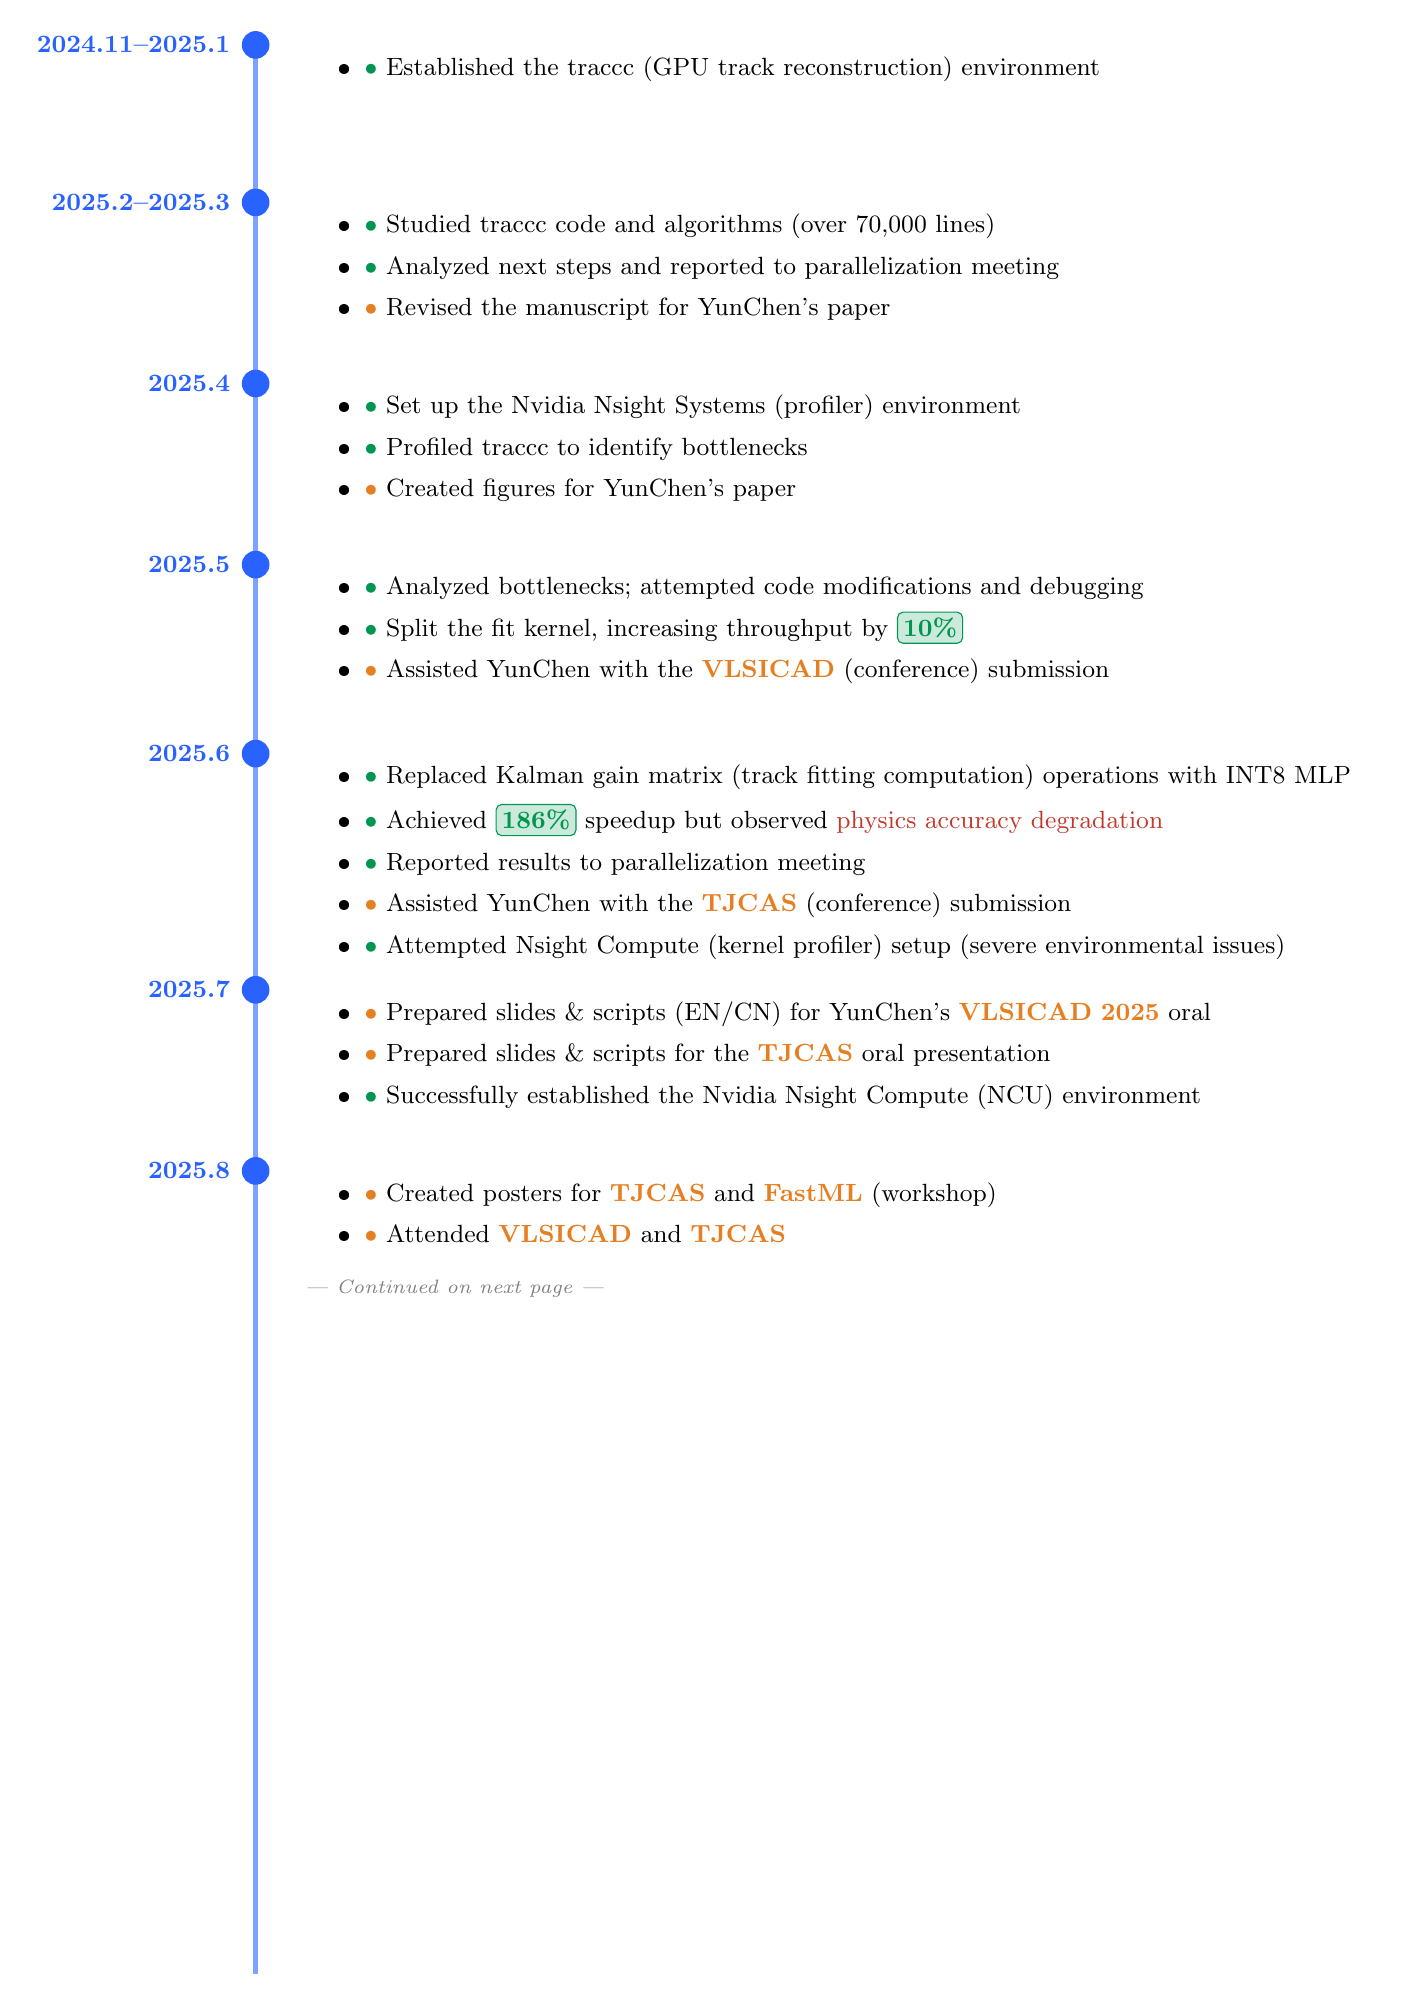
\begin{tikzpicture}[
  timeline/.style={line width=2pt, draw=timelineblue!60},
  datenode/.style={circle, fill=timelineblue, minimum size=10pt, inner sep=0},
  datelabel/.style={font=\bfseries\small, text=timelineblue, anchor=east},
  entrybox/.style={anchor=north west, text width=14cm, inner sep=0, font=\small},
]

% Timeline spine
\draw[timeline] (0, 0) -- (0, -24.5);

% ==================== 2024.11 - 2025.1 ====================
\node[datenode] at (0, 0) {};
\node[datelabel] at (-0.2, 0) {2024.11--2025.1};
\node[entrybox] at (0.5, 0.15) {
\begin{itemize}
  \item \optmark\ Established the traccc (GPU track reconstruction) environment
\end{itemize}
};

% ==================== 2025.2 - 2025.3 ====================
\node[datenode] at (0, -2) {};
\node[datelabel] at (-0.2, -2) {2025.2--2025.3};
\node[entrybox] at (0.5, -1.85) {
\begin{itemize}
  \item \optmark\ Studied traccc code and algorithms (over 70,000 lines)
  \item \optmark\ Analyzed next steps and reported to parallelization meeting
  \item \confmark\ Revised the manuscript for YunChen's paper
\end{itemize}
};

% ==================== 2025.4 ====================
\node[datenode] at (0, -4.3) {};
\node[datelabel] at (-0.2, -4.3) {2025.4};
\node[entrybox] at (0.5, -4.15) {
\begin{itemize}
  \item \optmark\ Set up the Nvidia Nsight Systems (profiler) environment
  \item \optmark\ Profiled traccc to identify bottlenecks
  \item \confmark\ Created figures for YunChen's paper
\end{itemize}
};

% ==================== 2025.5 ====================
\node[datenode] at (0, -6.6) {};
\node[datelabel] at (-0.2, -6.6) {2025.5};
\node[entrybox] at (0.5, -6.45) {
\begin{itemize}
  \item \optmark\ Analyzed bottlenecks; attempted code modifications and debugging
  \item \optmark\ Split the fit kernel, increasing throughput by \speedup{10\%}
  \item \confmark\ Assisted YunChen with the \conf{VLSICAD} (conference) submission
\end{itemize}
};

% ==================== 2025.6 ====================
\node[datenode] at (0, -9.0) {};
\node[datelabel] at (-0.2, -9.0) {2025.6};
\node[entrybox] at (0.5, -8.85) {
\begin{itemize}
  \item \optmark\ Replaced Kalman gain matrix (track fitting computation) operations with INT8 MLP
  \item \optmark\ Achieved \speedup{186\%} speedup but observed \warn{physics accuracy degradation}
  \item \optmark\ Reported results to parallelization meeting
  \item \confmark\ Assisted YunChen with the \conf{TJCAS} (conference) submission
  \item \optmark\ Attempted Nsight Compute (kernel profiler) setup (severe environmental issues)
\end{itemize}
};

% ==================== 2025.7 ====================
\node[datenode] at (0, -12.0) {};
\node[datelabel] at (-0.2, -12.0) {2025.7};
\node[entrybox] at (0.5, -11.85) {
\begin{itemize}
  \item \confmark\ Prepared slides \& scripts (EN/CN) for YunChen's \conf{VLSICAD 2025} oral
  \item \confmark\ Prepared slides \& scripts for the \conf{TJCAS} oral presentation
  \item \optmark\ Successfully established the Nvidia Nsight Compute (NCU) environment
\end{itemize}
};

% ==================== 2025.8 ====================
\node[datenode] at (0, -14.3) {};
\node[datelabel] at (-0.2, -14.3) {2025.8};
\node[entrybox] at (0.5, -14.15) {
\begin{itemize}
  \item \confmark\ Created posters for \conf{TJCAS} and \conf{FastML} (workshop)
  \item \confmark\ Attended \conf{VLSICAD} and \conf{TJCAS}
\end{itemize}
};

% ==================== Page break hint ====================
\node[font=\scriptsize\itshape, text=gray, anchor=west] at (0.5, -15.8) {--- Continued on next page ---};

\end{tikzpicture}

\newpage

% Continue timeline on page 2
\begin{tikzpicture}[remember picture, overlay]
  % Ongoing work sidebar continues on page 2
  \fill[ongoingblue, opacity=0.12, rounded corners=3pt]
    ([xshift=0.35in, yshift=-0.6in]current page.north east) rectangle
    ([xshift=0.05in, yshift=-8.5in]current page.north east);
  \node[rotate=90, font=\footnotesize\itshape, text=ongoingblue, anchor=south]
    at ([xshift=0.2in, yshift=-4.5in]current page.north east)
    {NCU Profile Flow Optimization (Ongoing)};
\end{tikzpicture}

\noindent
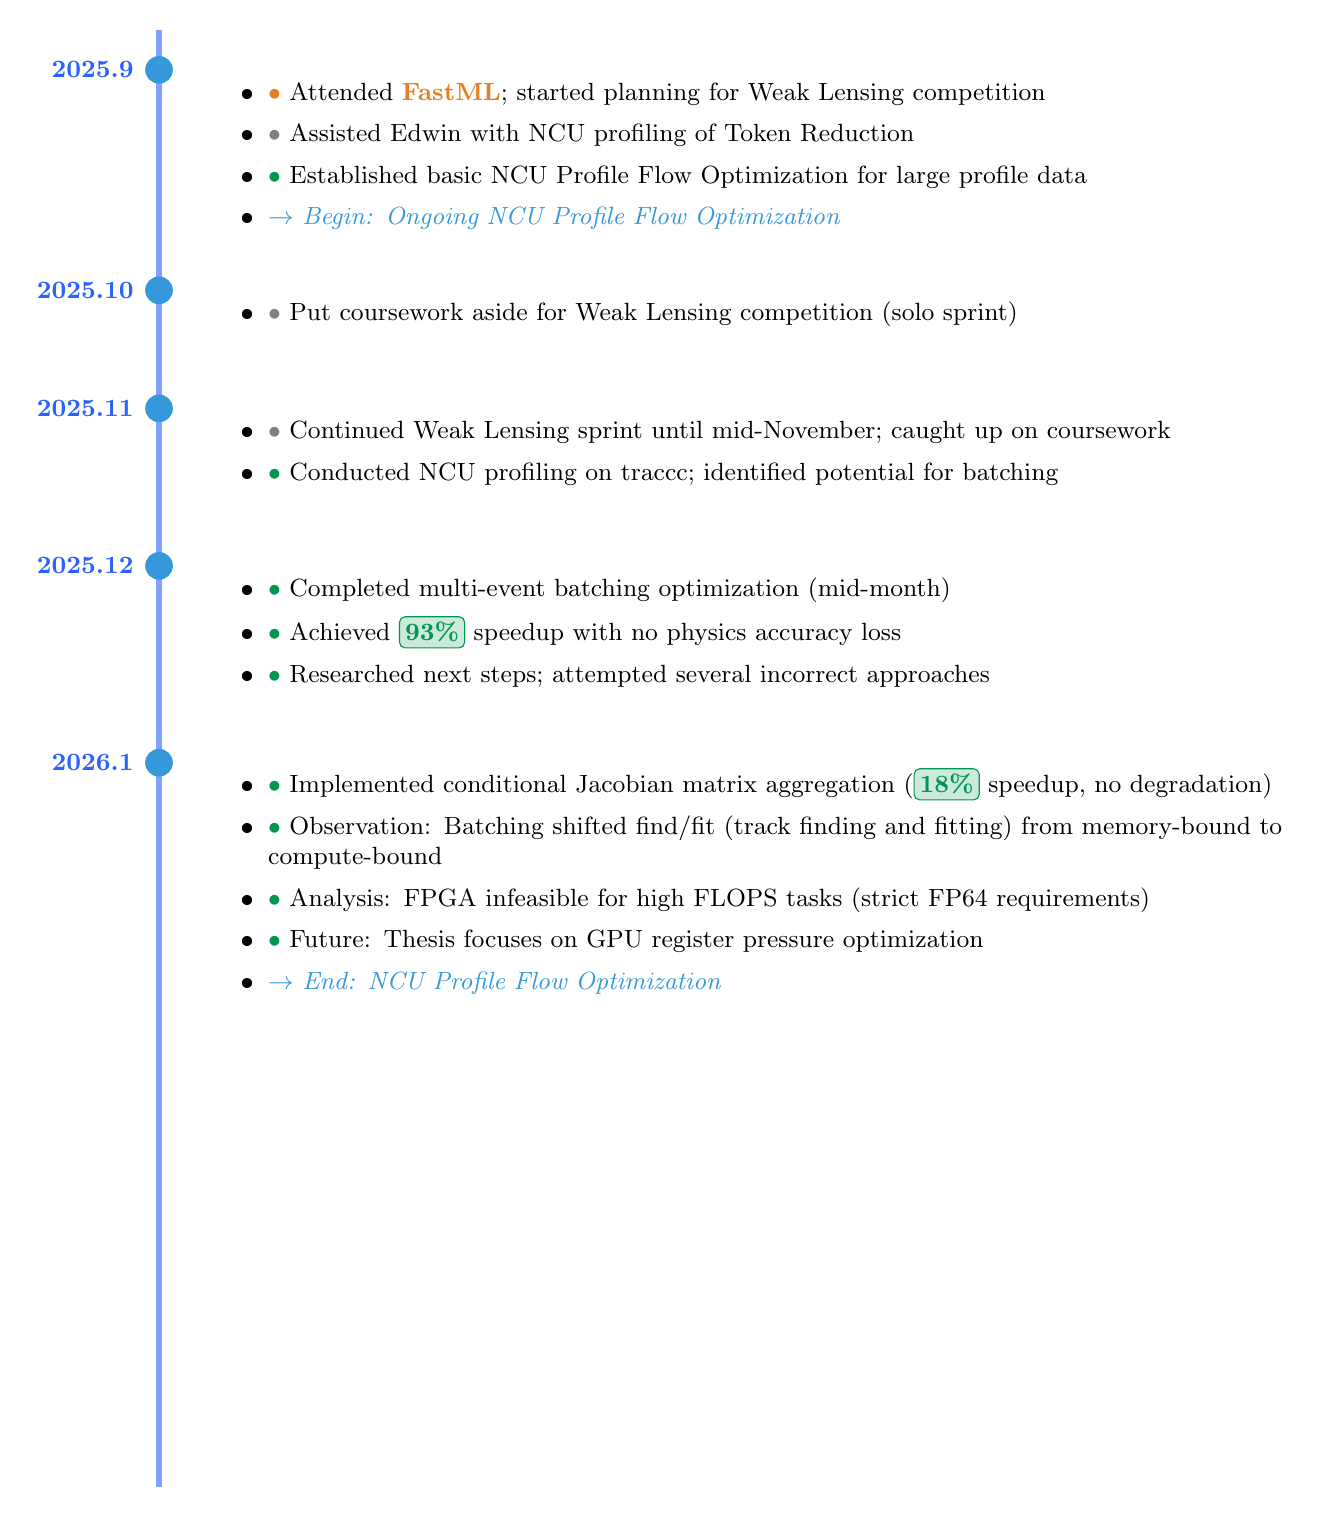
\begin{tikzpicture}[
  timeline/.style={line width=2pt, draw=timelineblue!60},
  datenode/.style={circle, fill=timelineblue, minimum size=10pt, inner sep=0},
  datenode ongoing/.style={circle, fill=ongoingblue, minimum size=10pt, inner sep=0},
  datelabel/.style={font=\bfseries\small, text=timelineblue, anchor=east},
  entrybox/.style={anchor=north west, text width=14cm, inner sep=0, font=\small},
]

% Timeline spine (page 2)
\draw[timeline] (0, 0.5) -- (0, -18);

% ==================== 2025.9 ====================
\node[datenode ongoing] at (0, 0) {};
\node[datelabel] at (-0.2, 0) {2025.9};
\node[entrybox] at (0.5, 0.15) {
\begin{itemize}
  \item \confmark\ Attended \conf{FastML}; started planning for Weak Lensing competition
  \item \collabmark\ Assisted Edwin with NCU profiling of Token Reduction
  \item \optmark\ Established basic NCU Profile Flow Optimization for large profile data
  \item \textit{\textcolor{ongoingblue}{$\rightarrow$ Begin: Ongoing NCU Profile Flow Optimization}}
\end{itemize}
};

% ==================== 2025.10 ====================
\node[datenode ongoing] at (0, -2.8) {};
\node[datelabel] at (-0.2, -2.8) {2025.10};
\node[entrybox] at (0.5, -2.65) {
\begin{itemize}
  \item \collabmark\ Put coursework aside for Weak Lensing competition (solo sprint)
\end{itemize}
};

% ==================== 2025.11 ====================
\node[datenode ongoing] at (0, -4.3) {};
\node[datelabel] at (-0.2, -4.3) {2025.11};
\node[entrybox] at (0.5, -4.15) {
\begin{itemize}
  \item \collabmark\ Continued Weak Lensing sprint until mid-November; caught up on coursework
  \item \optmark\ Conducted NCU profiling on traccc; identified potential for batching
\end{itemize}
};

% ==================== 2025.12 ====================
\node[datenode ongoing] at (0, -6.3) {};
\node[datelabel] at (-0.2, -6.3) {2025.12};
\node[entrybox] at (0.5, -6.15) {
\begin{itemize}
  \item \optmark\ Completed multi-event batching optimization (mid-month)
  \item \optmark\ Achieved \speedup{93\%} speedup with no physics accuracy loss
  \item \optmark\ Researched next steps; attempted several incorrect approaches
\end{itemize}
};

% ==================== 2026.1 ====================
\node[datenode ongoing] at (0, -8.8) {};
\node[datelabel] at (-0.2, -8.8) {2026.1};
\node[entrybox] at (0.5, -8.65) {
\begin{itemize}
  \item \optmark\ Implemented conditional Jacobian matrix aggregation (\speedup{18\%} speedup, no degradation)
  \item \optmark\ Observation: Batching shifted find/fit (track finding and fitting) from memory-bound to compute-bound
  \item \optmark\ Analysis: FPGA infeasible for high FLOPS tasks (strict FP64 requirements)
  \item \optmark\ Future: Thesis focuses on GPU register pressure optimization
  \item \textit{\textcolor{ongoingblue}{$\rightarrow$ End: NCU Profile Flow Optimization}}
\end{itemize}
};

\end{tikzpicture}

\vspace{1.5em}

% Legend
\noindent\rule{\textwidth}{0.4pt}
\vspace{0.5em}

\noindent\textbf{Legend}\\[0.3em]
\begin{tabular}{@{}lll@{}}
\optmark\ Technical/Optimization &
\confmark\ Conference/Paper &
\collabmark\ Collaboration/Other \\[0.5em]
\end{tabular}

\noindent
\speedup{Green Badge} = Performance Achievement \quad
\warn{Red Text} = Accuracy Concern \quad
\textcolor{ongoingblue}{Blue Sidebar} = NCU Flow Optimization Period

\vspace{0.3em}
\noindent\rule{\textwidth}{0.4pt}

% Key Achievements Summary
\vspace{0.8em}
\noindent\textbf{Key Performance Achievements}\\[0.3em]
\begin{tabular}{@{}lll@{}}
\speedup{10\%} & Fit kernel splitting & 2025.5 \\
\speedup{186\%} & INT8 MLP replacement (with accuracy trade-off) & 2025.6 \\
\speedup{93\%} & Multi-event batching (no accuracy loss) & 2025.12 \\
\speedup{18\%} & Conditional Jacobian aggregation (no accuracy loss) & 2026.1 \\
\end{tabular}

\vfill
\begin{center}
\small\textcolor{gray}{Generated: January 2026}
\end{center}

\end{document}
